\chapter{Singular Value Decomposition}

In the previous chapter you learned how to calculate eigenvalues and eigenvectors. But not every matrix has them. For those matrices, singular values and singular vectors are analogous features. 

Singular Value Decomposition (SVD) is a matrix factorization technique that breaks down a matrix into three matrices that represent the structure and properties of the original matrix.The decomposed matrices make calculations easier and provide insight into the original matrix. Basically, SVD can transform a high dimension, highly variable set of data into a set of uncorrelated data points that reveal subgroupings that you might not have noticed in the original data.
\index{singular value decomposition} \index{svd}


\section{Definition}

For any $m \times n$ matrix $A$, decomposes the matrix into three matrices.

\begin{equation}
A = U \Sigma V^T
\end{equation}

$U$ and $V$ are orthogonal matrices. \Sigma is a diagonal matrix that is the same size as $A$. Its diagonal contain the singular values of $A$. 

\begin{itemize}
\item $U$ is an orthogonal matrix whose size is $m \times m$. Its columns are the
  eigenvectors of $AA^T$. These are the left singular vectors of $A$. Because $U$ is orthogonal,$U^TU = I$
\item $V$ is an orthogonal matrix whose size is $n \times n$ matrix. Its columns are the
  eigenvectors of $A^TA$. These are the right singular vectors of $A$. Because $V$ is orthogonal, $V^TV = I$.
\item  \Sigma is a diagonal matrix that is the same size as $A$. Its diagonal contains the singular values of $A$, arranged in descending order. These values are the square roots of the eigenvalues of both $A^TA$ and  $AA^T$. 
\end{itemize}

\section{Applications of SVD}

SVD has numerous applications:

\begin{itemize}
\item It's used in machine learning and data science to perform
  dimensionality reduction, particularly through a technique known as
  Principal Component Analysis (PCA).

\item In numerical linear algebra, SVD is used to solve linear
  equations and compute matrix inverses in a more numerically stable
  way.

\item It's used in image compression, where low-rank approximations of
  an image matrix provide a compressed version of the original image.
\end{itemize}

\section{Calculating SVD Manually}
You might be inclined to skip this example because the computations are lengthy. Why would anyone do this when they can use a computing language, like Python, to calculate the SVD with essentially one command? We show this so you can understand what goes on "under the hood" when you compute SVD programmatically. 

After you read through this example, you'll see how to use Python to compute SVD. Then you'll see an example of using SVD for image compression. Finally, you'll have an exercise to compute the SVD. For this, you'll need to write your own Python script.

Let's find the SVD for matrix $A$. Recall that we want to find $U$. $\Sigma$, and $V^T$ such that:

\begin{equation}
A = U \Sigma V^T
\end{equation}

$$ A = \begin{bmatrix}
3,1,1 &  \\
 -1, 3,1& 
\end{bmatrix}$$

$$U = AA^T$$ 

Start with $A^T$:
$$ A^T = \begin{bmatrix}
3,-1 &  \\
1,3 &  \\
1,1& 
\end{bmatrix}$$
$$AA^T = \begin{bmatrix}
3,1,1 &  \\
 -1, 3,1& 
\end{bmatrix}
\begin{bmatrix}
3,-1 &  \\
1,3 &  \\
1,1& 
\end{bmatrix}
= \begin{bmatrix}
11,1 &  \\
 1, 11& 
\end{bmatrix}
$$
Next we will find the eigenvalues and eigenvectors of $A^T$. This is a chance to apply what you learned in the previous chapter. We know that:
\begin{equation}
Av = \lambda v
\end{equation}
So:
$$
\begin{bmatrix}
11,1 &  \\
 1, 11& 
\end{bmatrix}
\begin{bmatrix}
x_1 &  \\
x_2& 
\end{bmatrix}
=
\lambda 
\begin{bmatrix}
x_1 &  \\
x_2& 
\end{bmatrix}
$$
Rewrite as a set of equations:
$$11x_1 + x_2 = \lambda x_1$$
$$x_1 + 11x_2 = \lambda x_2$$
Then rearrange:
$$(11−\lambda )x_1 +x_2 =0$$
$$x_1 +(11−\lambda )x_2 =0 $$
Solve for \lambda :
$$\begin{bmatrix}
(11 -\lambda), 1 \\
 1, (11 -\lambda) 
\end{bmatrix} = 0$$
And as equations:
$$(11 − \lambda)(11 − \lambda) − 1 · 1 = 0$$
$$(\lambda − 10)(\lambda − 12) = 0$$
These are the eigenvalues.
$$\lambda = 10$$
$$\lambda = 12$$
When substituted into the original equations, you get the eigenvectors. For $$ \lambda = 10$$:
$$(11−10)x_1 +x_2 =0 $$
$$x_1 = -x_2$$
We'll set $$x_1$$ to 1 and get this eigenvector:
$$\left[ 1,-1 \right]$$
For $$ \lambda = 10$$:
$$(11−12)x_1 +x_2 =0  $$
$$x_1 = x_2 $$
We'll set $$x_1$$ to 1 and get this eigenvector:
$$\left[ 1,1 \right]$$
The matrix is:
$$
\begin{bmatrix}
1,1 \\
1,-1 
\end{bmatrix}
$$
Next you need to apply the Gram-Schmidt process to the column vectors. Then you'll have $U$, the $m \times m$ matrix whose columns are eigenvectors of $AA^T$. These are the left singular vectors of $A$. After you apply Gram-Schmidt, you should end up with:
$$
U = \begin{bmatrix}
1/\sqrt{2},1/\sqrt{2} \\
1/\sqrt{2},-1/\sqrt{2} 
\end{bmatrix}
$$
The process for calculating $V$ is the same as the calculation for $U$, except:
$$V = A^TA$$ 
$$A^TA = 
\begin{bmatrix}
3,-1 &  \\
1,3 &  \\
1,1& 
\end{bmatrix}
\begin{bmatrix}
3,1,1 &  \\
 -1, 3,1& 
\end{bmatrix}
=
\begin{bmatrix}
10,0,2 \\
0,10,4 \\
 2,4,2
\end{bmatrix}
$$
After applying the process we applied to solve for U, you get:
$$
V = \begin{bmatrix}
1/\sqrt{6},2/\sqrt{5},1/\sqrt{30} \\
2/\sqrt{6},-1/\sqrt{5},2/\sqrt{30}\\
1/\sqrt{6},0,-5/\sqrt{30}
\end{bmatrix}
$$
However, you want $V_T$:
$$
V_T =
\begin{bmatrix}
1/\sqrt{6},2/\sqrt{6},1/\sqrt{6} \\
2/\sqrt{5},-1/\sqrt{5},0\\
1/\sqrt{30},2/\sqrt{30},-5/\sqrt{30}
\end{bmatrix}
$$
You have only to calculate $\Sigma$, a diagonal matrix that is the same size as $A$. The diagonal contains the singular values of $A$, arranged in descending order. They are the square roots of the eigenvalues of both $A^TA$ and  $AA^T$.

Because the non-zero eigenvalues of U are the same as V, let's use the eigenvalues we calculate for U, 10 and 12. Note that $\Sigma$ will not be of the correct dimension to reconstruct the orignal matrix unless we add a column. By adding a zero column you'll be able to multiply between $U$ and $V$:
$$
\Sigma = 
\begin{bmatrix}
\sqrt{12}, &0,&0\\
 0,&\sqrt{12}  &0 
\end{bmatrix}
$$
You can check your work by multiplying the decomposed matrices. This should return the orginal matrix.
$$A = U\Sigma V^T $$
$$ = 
U = \begin{bmatrix}
1/\sqrt{2},1/\sqrt{2} \\
1/\sqrt{2},-1/\sqrt{2} 
\end{bmatrix}
\begin{bmatrix}
\sqrt{12}, &0,&0\\
 0,&\sqrt{12}  &0 
\end{bmatrix}
\begin{bmatrix}
1/\sqrt{6},2/\sqrt{6},1/\sqrt{6} \\
2/\sqrt{5},-1/\sqrt{5},0\\
1/\sqrt{30},2/\sqrt{30},-5/\sqrt{30}
\end{bmatrix}
$$
$$=
\begin{bmatrix}
\sqrt{12}/\sqrt{2}, &\sqrt{10}/\sqrt{2},&0\\
\sqrt{12}/\sqrt{2},&-\sqrt{10}/\sqrt{2} &0 
\end{bmatrix}
\begin{bmatrix}
1/\sqrt{6}, &2/\sqrt{6},&1/\sqrt{6}\\
2/\sqrt{5},&-1/\sqrt{5} &0 \\
1/\sqrt{30},&2/\sqrt{30},&-5/\sqrt{30}
\end{bmatrix}
$$
$$
=
\begin{bmatrix}
3,1,1 &  \\
 -1, 3,1& 
\end{bmatrix}
$$ 

\section{Singular Value Decomposition with Python}
Create a file called \filename{vectors\_decomposition.py} and enter this code:

\begin{Verbatim}
# Singular-value decomposition
import numpy as np
from numpy import array
from scipy.linalg import svd
from numpy import diag
from numpy import dot
from numpy import zeros

# Define a matrix
A = array([[1, 2], [3, 4], [5, 6]])

print("Matrix (3x2) to be decomposed: ")
print(A)

# CalculateSVD
U, S, VT = svd(A)
print("Matrix (3x3) that represents the left singular values of A:")
print(U)
print("Singular values:")
print(S)
print("Matrix (2x2) that represents the right singular values of A:")
print(VT)

# Check if the decomposition by rebuilding the original matrix
# The singular values must be in an m x n matrix 
# Create a zero matrix with the same dimension as A
Sigma = zeros((A.shape[0], A.shape[1]))
# Populate Sigma with n x n diagonal matrix
Sigma[:A.shape[1], :A.shape[1]] = diag(S)
# Reconstruct the original matrix
A_Rebuilt = U.dot(Sigma.dot(VT))
print("Original matrix:")
print(A_Rebuilt)
\end{Verbatim}

\section{Sign Ambiguity}
You might notice that at times the absolute values in the $U$ and $V^T$ matrices are correct but that the signs vary from what you see as the answer. For example, when you compare a manually calculated SVD with one done in Python the signs might not agree. Both decompositions a $A$ are valid. Both decompositions will satisfy:
$$A = U \Sigma V^T$$
Note that the $S$ diagonal values will always be positive. 

The sign ambiguity has implications. For example, when using SVD to compress data, if some of the signs are flipped, the data can have artifacts. At this point in your education, you don't need to concern yourself with it except when you are comparing SVD results for the same matrix.

\begin{Exercise}[title={Single Value Decomposition}, label=svd]
Modify your Python code to calculate SVD for the matrix in the worked out example. Did yo arrive at the same answer? Keep in mind that Python will compute square roots and present fractions as decimal. Take a look at the signs for the values in the $U$ and $V^T$ matrices. Are they the same or is this an example of sign ambiguity? 
\end{Exercise}
\begin{Answer}[ref=svd]
$$U = 
\begin{bmatrix}
-0.70710678 &-0.70710678  \\
 -0.70710678 &0.70710678 
\end{bmatrix}
$$
$$Singular values = [3.46410162 3.16227766]
$$
$$V^T =
\begin{bmatrix}
 -0.408 &-0.816  &-0.408  \\
 -0.894 &0.447 &0.0  \\
 -0.183 &-0.365  &0.9129 
\end{bmatrix}
$$
\end{Answer}

\section{SVD Applied to Image Compression}
This image consists of a grid of 20 by 10 pixels, each of which is either black or white.

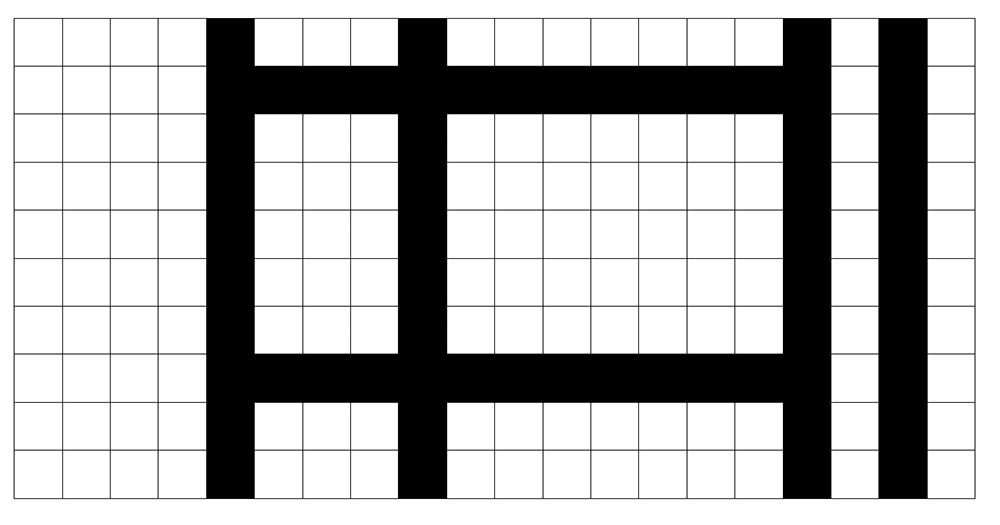
\includegraphics[width=0.4\textwidth]{ImageCompress.png}

It's a simple image that has only two types of columns--ideal for data compression. A row is either the first pattern or the second.

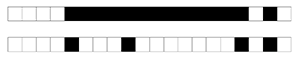
\includegraphics[scale=0.8]{Rows.png}

We can represent the data as a 20 by 10 matrix whose 200 entries are either 0 for black or 1 for white. 
$$
\begin{bmatrix}
0 0 0 0 1 0 0 0 1 0 0 0 0 0 0 0 1 0 1 0\\
0 0 0 0 1 1 1 1 1 1 1 1 1 1 1 1 1 0 1 0\\
0 0 0 0 1 0 0 0 1 0 0 0 0 0 0 0 1 0 1 0\\
0 0 0 0 1 0 0 0 1 0 0 0 0 0 0 0 1 0 1 0\\
0 0 0 0 1 0 0 0 1 0 0 0 0 0 0 0 1 0 1 0\\
0 0 0 0 1 0 0 0 1 0 0 0 0 0 0 0 1 0 1 0\\
0 0 0 0 1 0 0 0 1 0 0 0 0 0 0 0 1 0 1 0\\
0 0 0 0 1 1 1 1 1 1 1 1 1 1 1 1 1 0 1 0\\
0 0 0 0 1 0 0 0 1 0 0 0 0 0 0 0 1 0 1 0\\
0 0 0 0 1 0 0 0 1 0 0 0 0 0 0 0 1 0 1 0
\end{bmatrix}
$$
When you perform an SVD on this matrix, there are only two non-zero singular values, 6.79 and 3.72. (You are welcome perform the calculation in Python.) Thus you can represent the matrix as:
$$
A = U_1 S_1 V_1 + U_2 S_2 V_2
$$
This means there are two $u$ vectors each with 20 entries and two $v$ vectors each with 10 entries, and two singular values. Add those up: 2*20 + 2*10 + 2 = 62. This implies that the image can be represented by 62 values instead of 200. If you look back at the image, you can see that there are many dependent columns and very few independent ones. 

This is a simple image and a small pixel matrix. But it should give you a sense of how SVD can decompose an image in a way that identifies how much of the image is redundant, and therefor can be compressed.

\section{Where to Learn More}
\emph {We Recommend a Singular Value Decomposition}. This American Mathematical Society publication focuses the geometry of SVD. What I like about the article is that it  shows both graphically and numerically how SVD can be used for data compression on images and for noise reduction. The data compression example in your workbook is based on this article. https://www.ams.org/publicoutreach/feature-column/fcarc-svd

\emph {Sign Ambiguity in Singular Value Decomposition (SVD)}. This is a good article for those who want a deeper understanding of sign ambiguity. https://www.educative.io/blog/sign-ambiguity-in-singular-value-decomposition

\emph {Singular Value Decomposition Tutorial}. This PDF starts by defining points, space, and vectors and works through all the concepts you need to tackle SVD. It is one of the few resources that has a completely worked out example of manually calculating SVD. The example in this chapter is from that tutorial. If you read the entire paper, you'll find it is a good review of the concepts you've studied in previous chapters. 
